\newlength{\textwidthMultiplier}
\setlength{\textwidthMultiplier}{0.45\textwidth}

This section presents the results obtained from evaluating the performance of the SimpleModel and DeepModel under various configurations, focusing on feature selection strategies, learning rates, optimizers, and gradient clipping techniques. The key performance metrics, including MAE, MAPE, and MSE, are used to assess and compare the models' effectiveness in minimizing the force error between the simulated and experimental results.

\subsection{Conducted Tests}

This section presents the performance evaluation of SimpleModel and DeepModel across the three previously introduced feature selection strategies. Each configuration is run for 600 epochs to ensure comparability. The learning rate is set at either 0.0005 or 0.001, with RMSprop used for the \textit{Regularization} configuration and Adam for the \textit{No Selector} and \textit{Enforce Direction} configurations. Gradient clipping values of 5, 10, and 15 are used for Regularization, No Selector, and Enforce Direction, respectively. These configurations are selected based on previous experiments to optimize the models' performance and to facilitate a balanced comparison.

\begin{table}[h]
    \centering
    \begin{tabular}{|c|c|c|c|c|c|}
        \hline
        \textbf{Model} & \textbf{Feature Selector} & \textbf{Learn rate (lr/{$\boldsymbol\mu$)}} & \textbf{Optimizer} & \textbf{Clipping Value} & \textbf{Epochs} \\ \hline
        SimpleModel & No Selector        & 0.001              & Adam      & 10             & 600    \\ \hline
        SimpleModel & Regularization     & 0.0005 / 0.001     & RMSprop   & 5              & 600    \\ \hline
        SimpleModel & Enforce Direction  & 0.001              & Adam      & 15             & 600    \\ \hline
        DeepModel   & No Selector        & 0.001              & Adam      & 10             & 600    \\ \hline
        DeepModel   & Regularization     & 0.0005 / 0.001     & RMSprop   & 5              & 600    \\ \hline
        DeepModel   & Enforce Direction  & 0.001              & Adam      & 15             & 600    \\ \hline
    \end{tabular}
    \caption{Comparison of SimpleModel and DeepModel across different feature selectors, learning rates, optimizers, and gradient clipping values.}
    \label{tab:configurations}
\end{table}



\subsection{Key Performance Metrics}
For the performance evaluation following metrics are used: The mean absolute error (MAE), the mean percentage error (MAPE) and the mean square error (MSE).Key performance metrics (KPM):
Lower Scalar results for all performance metrics mean "better results" in Terms of minimizing the force error between simulated and experimental force.

\begin{align*}
\text{MAE}(F_{\text{exp}}, F_{\text{sim}}) := \frac{1}{n} \sum_{i=1}^{n} |F_{\text{exp},i} - F_{\text{sim},i}|
\\
\text{MAPE}(F_{\text{exp}}, F_{\text{sim}}) := \frac{100\%}{n} \sum_{i=1}^{n} \left| \frac{F_{\text{exp},i} - F_{\text{sim},i}}{F_{\text{exp},i}} \right|
\\
\text{MSE}(F_{\text{exp}}, F_{\text{sim}}) := \frac{1}{n} \sum_{i=1}^{n} \left(F_{\text{exp},i} - F_{\text{sim},i}\right)^2.
\end{align*}



\subsection{Training}


\begin{table}[h!]
\centering
\caption{Performance metrics for different models and feature Selectors (rounded to 3 digits)}
\begin{tabular}{|l|l|l|c|>{\columncolor[gray]{0.9}}c|>{\columncolor[gray]{0.8}}c|>{\columncolor[gray]{0.7}}c|}
\hline
\textbf{Feature Selector} & \textbf{Model} & \textbf{Learn Rate} & \textbf{Epoch at Lowest Loss} & \textbf{MSE} & \textbf{MAPE} & \textbf{MAE} \\ \hline
EnforceS33Direction & DeepModel  & LR0005  & n.a.\footnotemark & $6.31 \times 10^2$ & 74.4 & 21.21 \\ \hline
EnforceS33Direction & DeepModel  & LR001  & 258 & $1.81 \times 10^3$ & 57.9 & 34.7 \\ \hline
Regularization      & DeepModel  & LR001  & 69  & $1.94 \times 10^3$ & 41.5 & 36.6 \\ \hline
Regularization      & DeepModel  & LR0005 & 581 & $3.66 \times 10^3$ & 52.8 & 53.0 \\ \hline
EnforceS33Direction & SimpleModel & LR001  & 590 & $5.70 \times 10^3$ & 63.2 & 64.4 \\ \hline
Regularization      & SimpleModel & LR0005 & 538 & $1.40 \times 10^4$ & 93.0 & 102 \\ \hline
Regularization      & SimpleModel & LR001  & 304 & $1.86 \times 10^4$ & 91.1 & 118 \\ \hline
EnforceS33Direction & SimpleModel & LR0005 & 516 & $1.90 \times 10^4$ & 85.2 & 121 \\ \hline
StandardFilter      & DeepModel  & LR001  & 535 & $1.62 \times 10^5$ & 293 & 291 \\ \hline
StandardFilter      & SimpleModel & LR001  & 599 & $1.73 \times 10^5$ & 239 & 374 \\ \hline
\end{tabular}
\label{tab:performance_metrics_training}
\end{table}

\footnotetext{n.a.: Data point not available for this entry.}




\begin{figure}[H]
    \centering
    
    % Title for the figure
    \caption*{\textbf{Training Results for No Selector}}

    % First set: Training No Selector
    \begin{subfigure}[b]{0.45\textwidth}
        \centering
        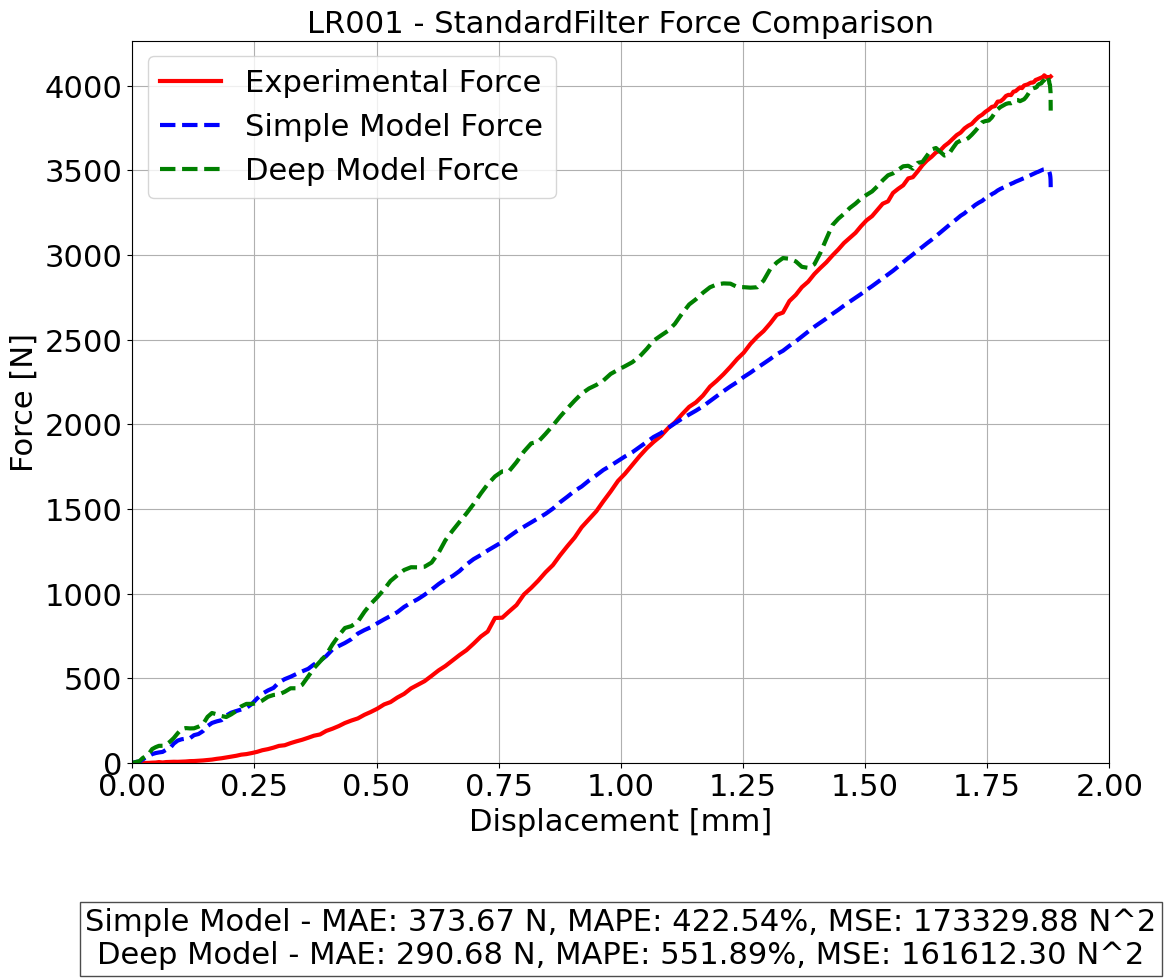
\includegraphics[width=\textwidth]{result_graphics/LR001_StandardFilter_Force_Comparison.png}
        \caption{Force Comparison}
        \label{fig:Training_No_Selector_Force}
    \end{subfigure}
    \hfill
    \begin{subfigure}[b]{0.45\textwidth}
        \centering
        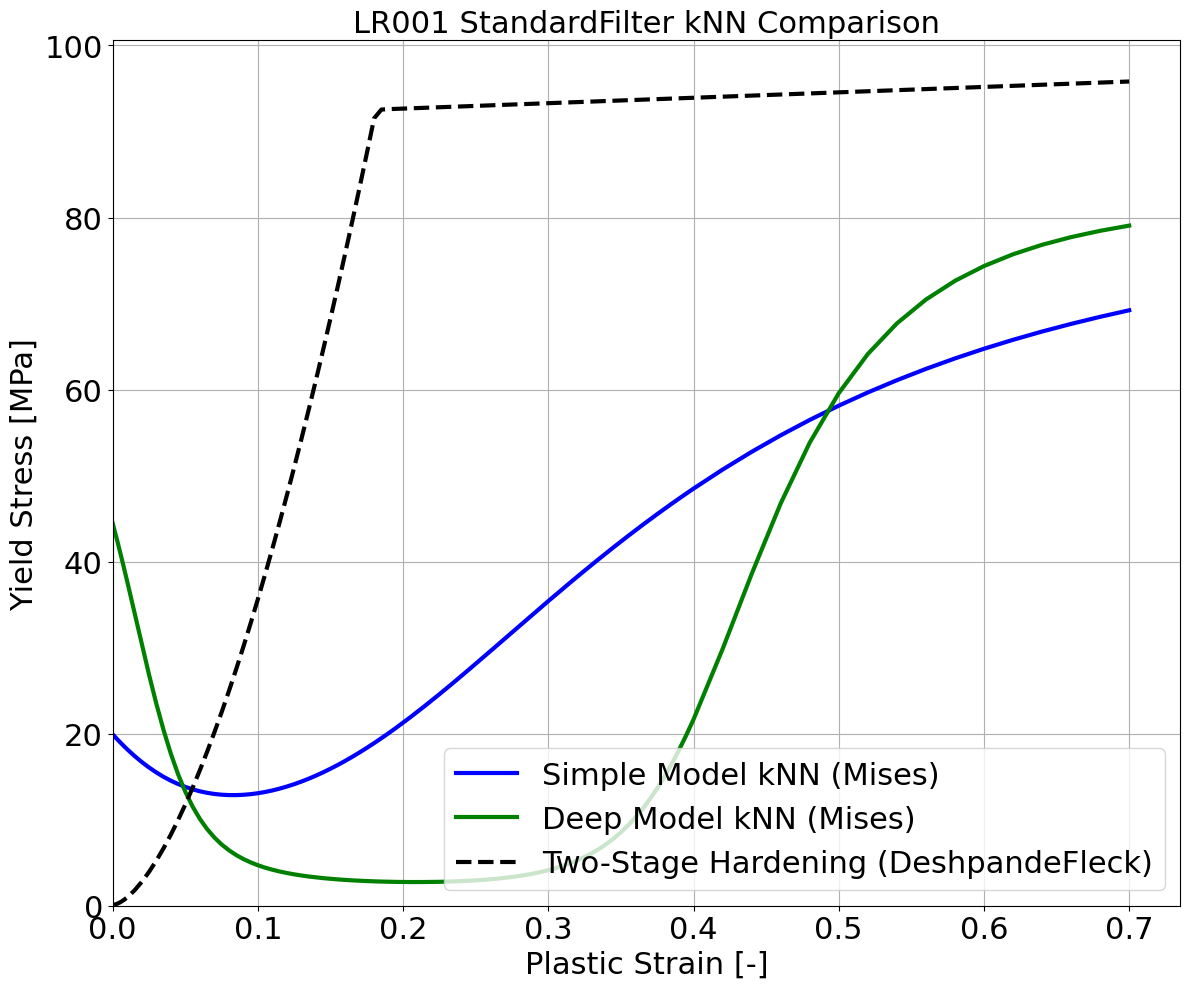
\includegraphics[width=\textwidth]{result_graphics/LR001_StandardFilter_kNN_Comparison_kNN_Comparison.png}
        \caption{kNN Comparison}
        \label{fig:Training_No_Selector_kNN}
    \end{subfigure}

    \caption{Training results without feature selector (No Selector) at LR 0.001.}
    \label{fig:Training_No_Selector}
\end{figure}

\begin{figure}[H]
    \centering
    
    % Title for the figure
    \caption*{\textbf{Training Results for Regularization}}

    % First set: Training Regularization LR 0.001
    \begin{subfigure}[b]{0.45\textwidth}
        \centering
        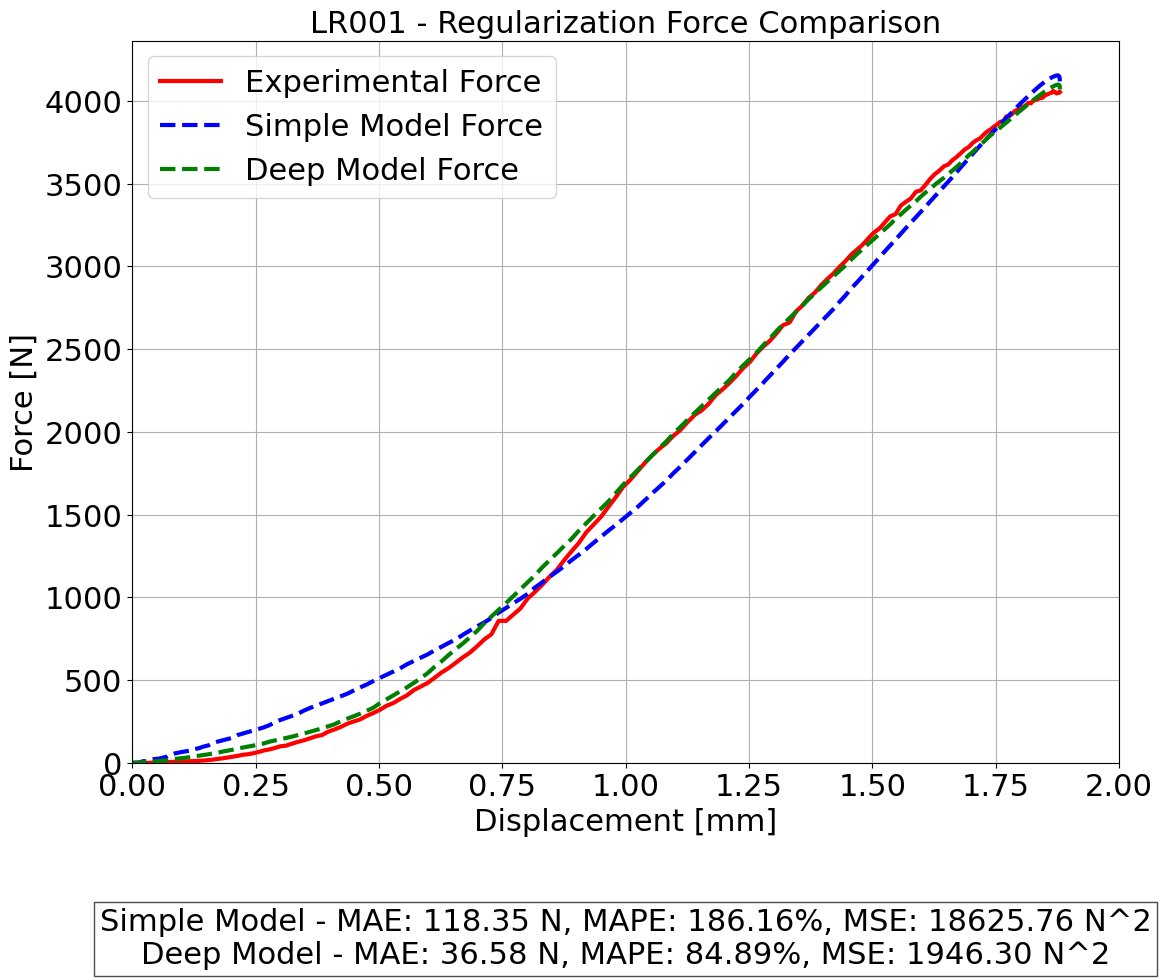
\includegraphics[width=\textwidth]{result_graphics/LR001_Regularization_Force_Comparison.png}
        \caption{Force Comparison for LR 0.001}
        \label{fig:Training_Regularization_001_Force}
    \end{subfigure}
    \hfill
    \begin{subfigure}[b]{0.45\textwidth}
        \centering
        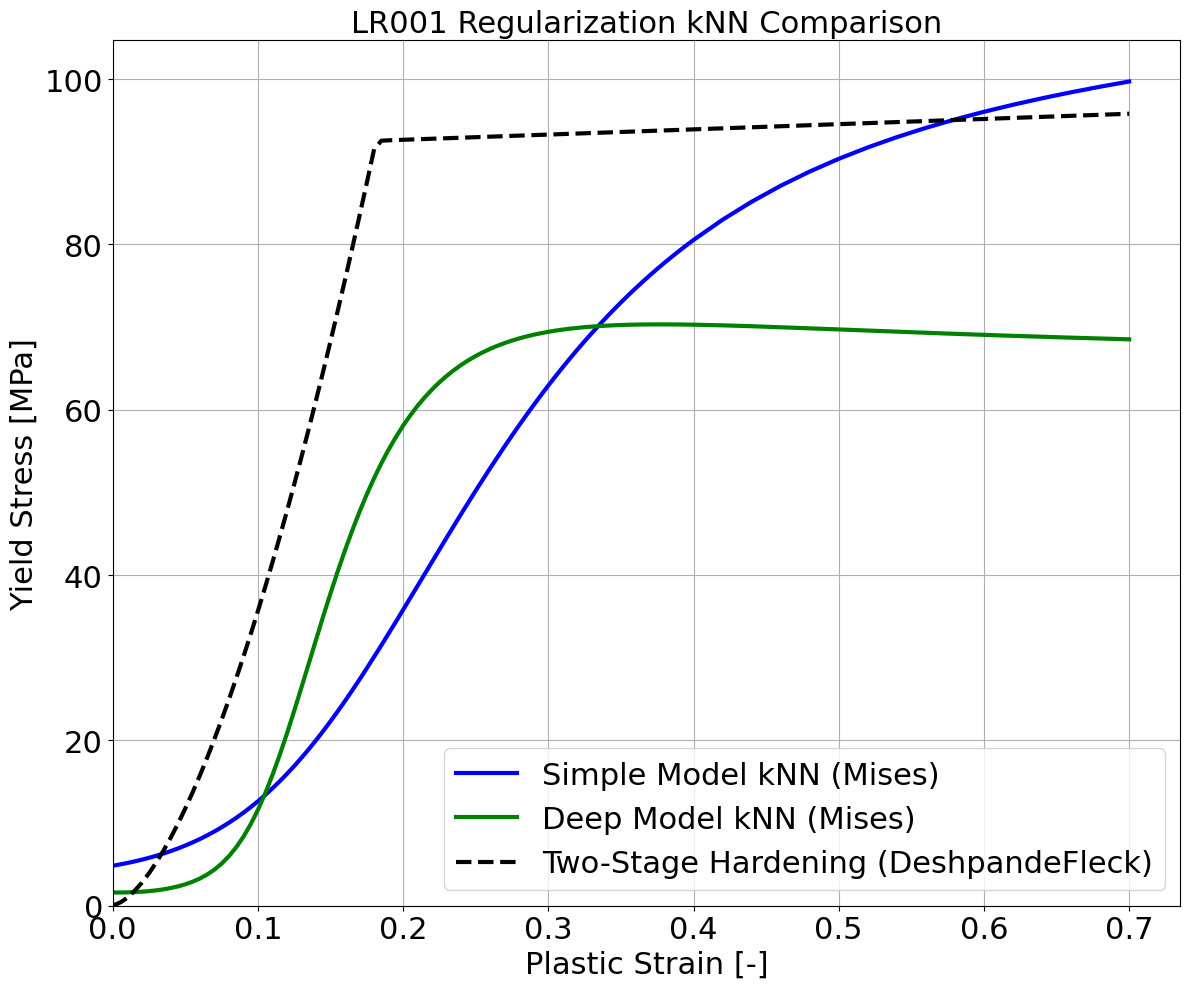
\includegraphics[width=\textwidth]{result_graphics/LR001_Regularization_kNN_Comparison_kNN_Comparison.png}
        \caption{kNN Comparison for LR 0.001}
        \label{fig:Training_Regularization_001_kNN}
    \end{subfigure}

    \vspace{1em}

    % Second set: Training Regularization LR 0.0005
    \begin{subfigure}[b]{0.45\textwidth}
        \centering
        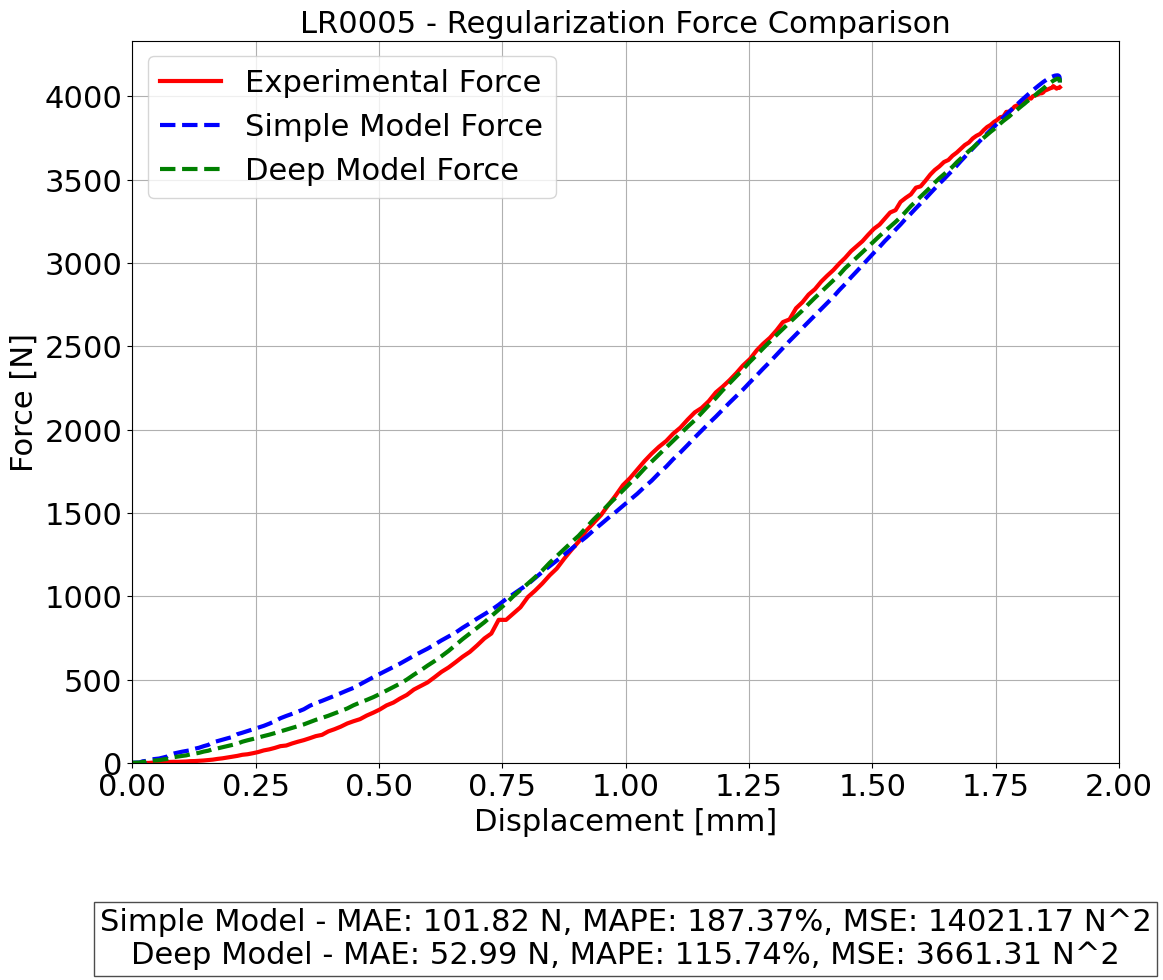
\includegraphics[width=\textwidth]{result_graphics/LR0005_Regularization_Force_Comparison.png}
        \caption{Force Comparison for LR 0.0005}
        \label{fig:Training_Regularization_0005_Force}
    \end{subfigure}
    \hfill
    \begin{subfigure}[b]{0.45\textwidth}
        \centering
        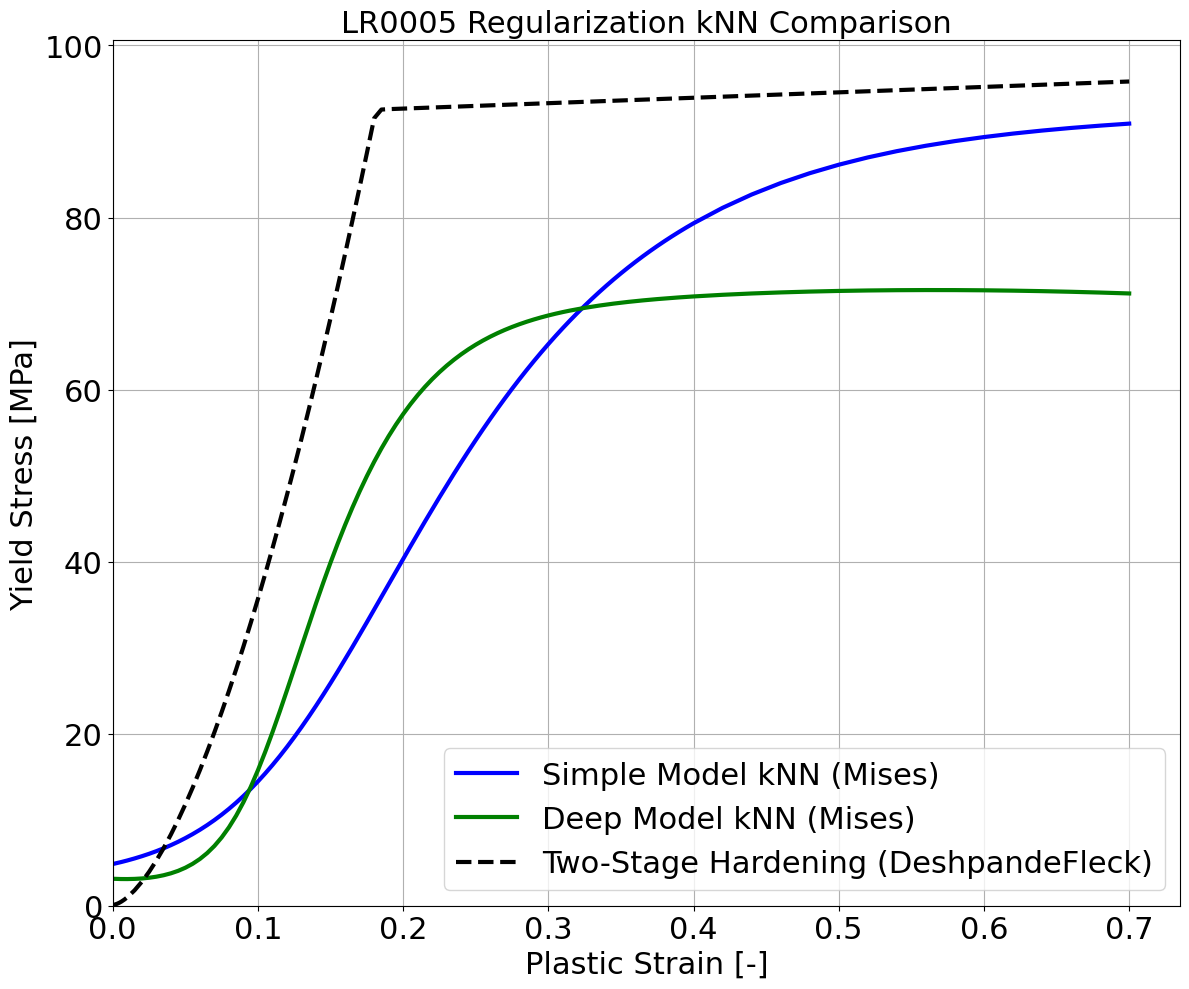
\includegraphics[width=\textwidth]{result_graphics/LR0005_Regularization_kNN_Comparison_kNN_Comparison.png}
        \caption{kNN Comparison for LR 0.0005}
        \label{fig:Training_Regularization_0005_kNN}
    \end{subfigure}

    \caption{Training results with regularization at different learning rates (LR 0.001 and LR 0.0005).}
    \label{fig:Training_Regularization}
\end{figure}

\begin{figure}[H]
    \centering
    
    % Title for the figure
    \caption*{\textbf{Training Results for Enforce Direction}}

    % First set: Training Enforce Direction LR 0.001
    \begin{subfigure}[b]{0.45\textwidth}
        \centering
        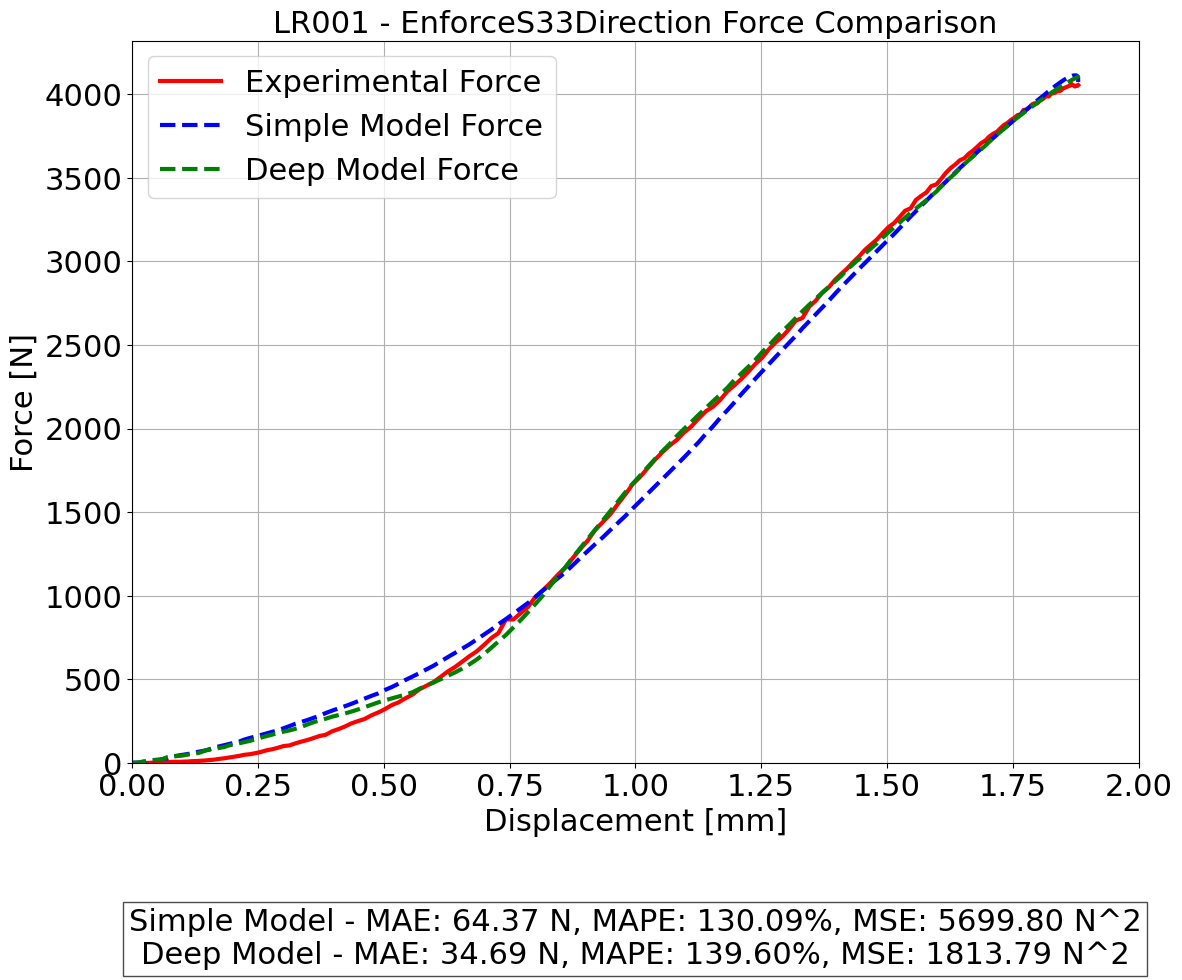
\includegraphics[width=\textwidth]{result_graphics/LR001_EnforceS33Direction_Force_Comparison.png}
        \caption{Force Comparison for LR 0.001}
        \label{fig:Training_Enforce_001_Force}
    \end{subfigure}
    \hfill
    \begin{subfigure}[b]{0.45\textwidth}
        \centering
        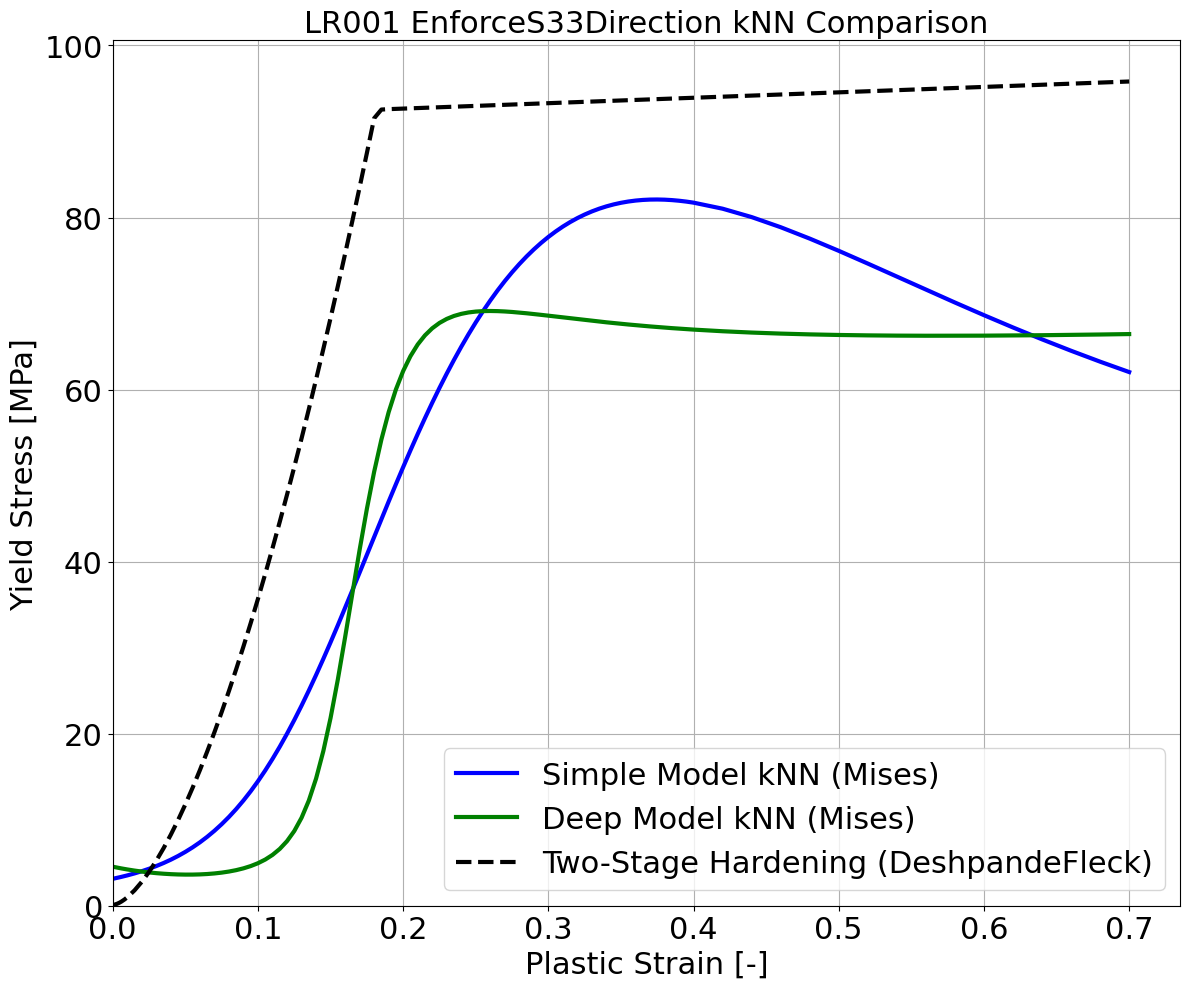
\includegraphics[width=\textwidth]{result_graphics/LR001_EnforceS33Direction_kNN_Comparison_kNN_Comparison.png}
        \caption{kNN Comparison for LR 0.001}
        \label{fig:Training_Enforce_001_kNN}
    \end{subfigure}

    \vspace{1em}

    % Second set: Training Enforce Direction LR 0.0005
    \begin{subfigure}[b]{0.45\textwidth}
        \centering
        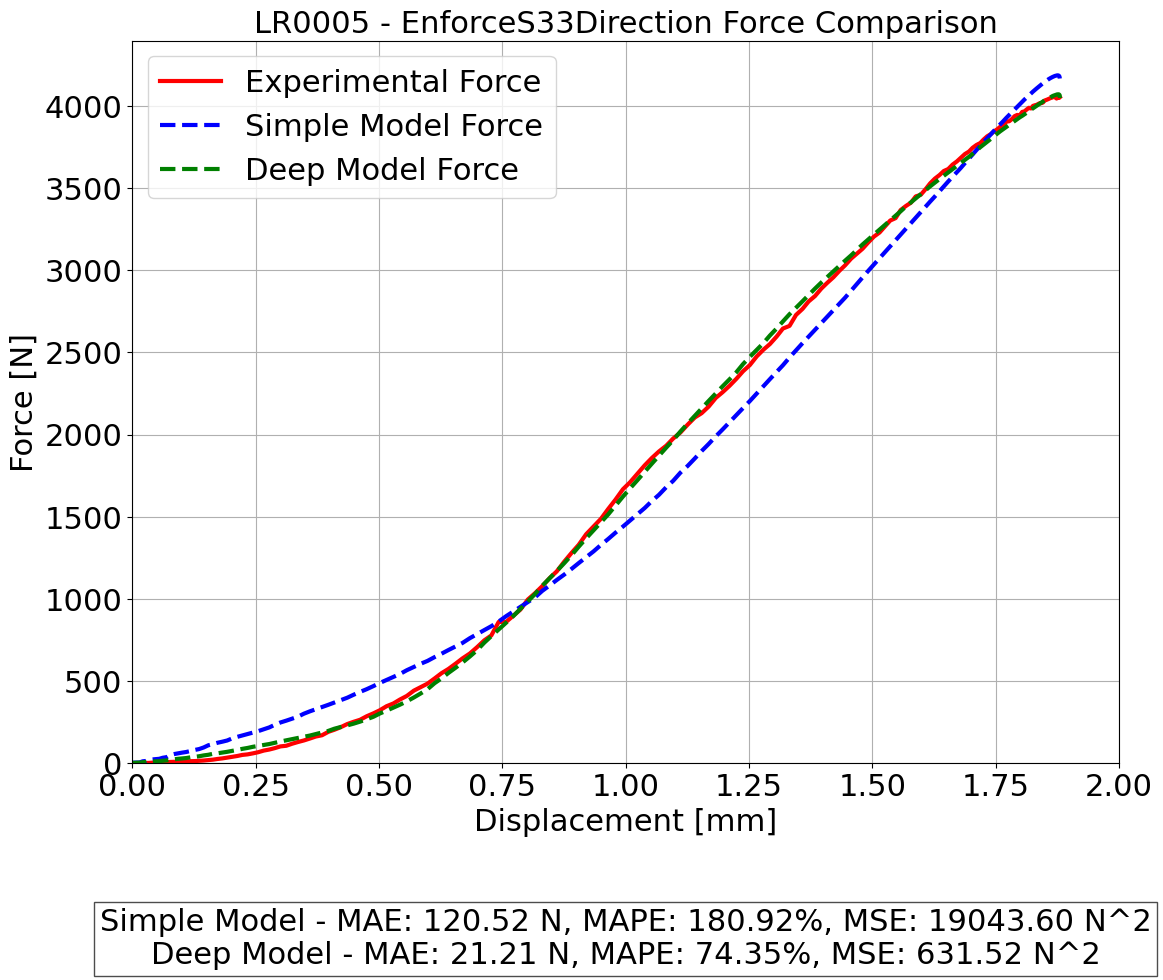
\includegraphics[width=\textwidth]{result_graphics/LR0005_EnforceS33Direction_Force_Comparison.png}
        \caption{Force Comparison for LR 0.0005}
        \label{fig:Training_Enforce_0005_Force}
    \end{subfigure}
    \hfill
    \begin{subfigure}[b]{0.45\textwidth}
        \centering
        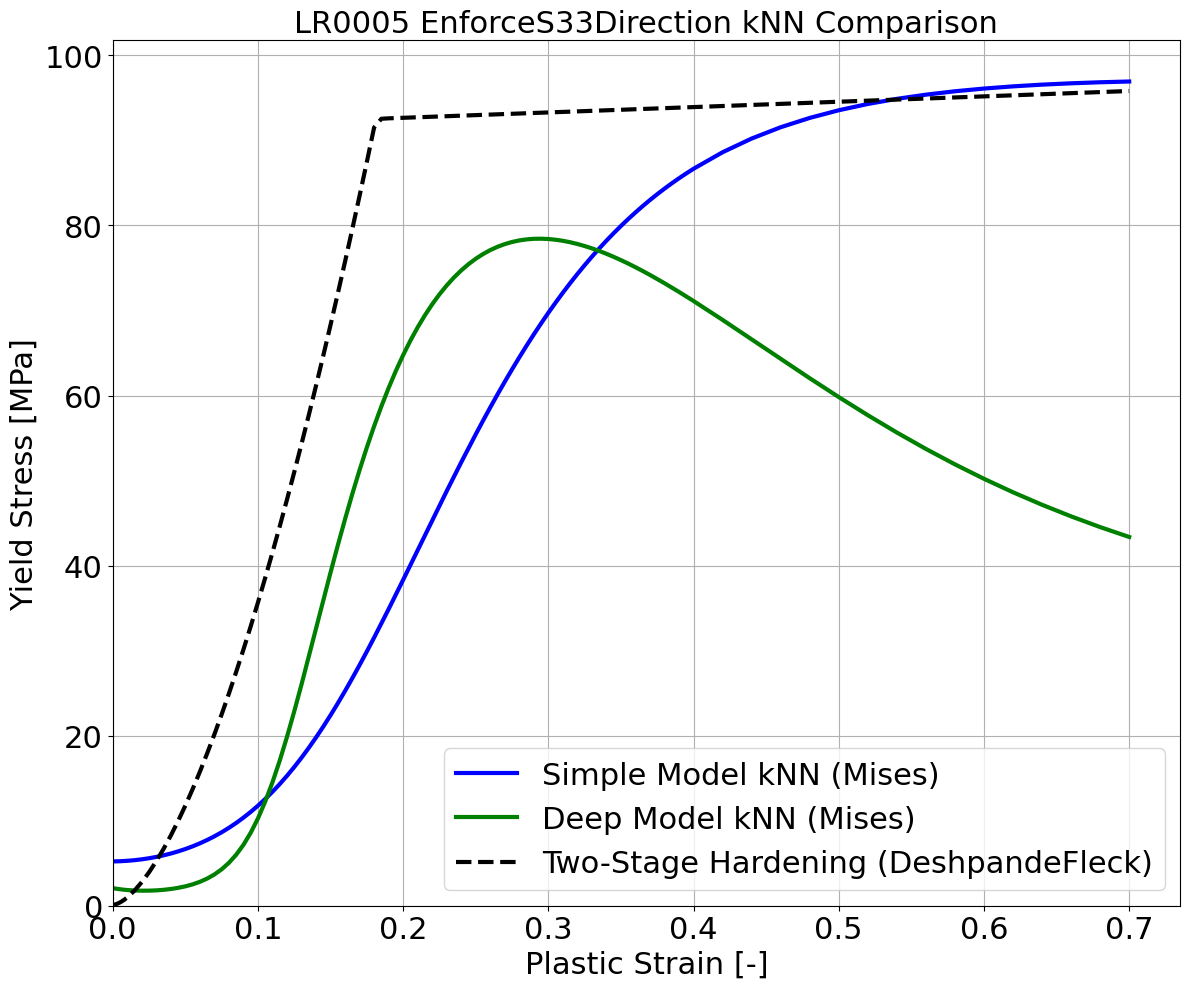
\includegraphics[width=\textwidth]{result_graphics/LR0005_EnforceS33Direction_kNN_Comparison_kNN_Comparison.png}
        \caption{kNN Comparison for LR 0.0005}
        \label{fig:Training_Enforce_0005_kNN}
    \end{subfigure}

    \caption{Training results with Enforce Direction at different learning rates (LR 0.001 and LR 0.0005).}
    \label{fig:Training_Enforce}
\end{figure}






The Key Performance Metrics and respective configurations of training runs are indicated in Table \ref{tab:performance_metrics_training}.
Figures
\ref{fig:Training_No_Selector},
\ref{fig:Training_Regularization},
\ref{fig:Training_Enforce}
show the training results for the specified method combinations. For shape comparison the two stage hardening law is included. The amplitude is not comparable as it was calibrated on a Deshpande-Fleck yield surface. Displayed are the results for the epoch, out of the total 600 epochs, that yield the lowest loss (MSE).

Further the MSE, MAPE and MAE for specified epochs and training combinations is displayed in the table.  The best run, based on the lowest performance metrics, was achieved by DeepModel with a learning rate of 0.005 and the Enforce Direction feature selector.

In contrast, the worst performance across all key performance metrics (KPM) was observed with DeepModel using a learning rate of 0.001 and the No Selector method. Overall, DeepModel with a learning rate of 0.005 and the Enforce Direction feature selector consistently produced the best results, minimizing error metrics across MSE and MAE performance measures.

The described simulations took 8 hours, running on Euler HPC, yielding a runtime of aproximately one minute per epoch.

DeepModel consistently performs better than SimpleModel, as presented in figures
\ref{fig:Training_No_Selector},
\ref{fig:Training_Regularization},
\ref{fig:Training_Enforce}
for the training runs on the H\_10 indenter except for the No Selector method. DeepModel predicted hardening laws with regularization and enforce direction are chosen to be validated on the H\_50 and C\_20 indenters. Regularization models are used as they show lower MAPE.

\subsection{Validation}


\begin{table}[H]
\centering
\begin{tabular}{|l|l|c|c|>{\columncolor[gray]{0.9}}c|>{\columncolor[gray]{0.8}}c|>{\columncolor[gray]{0.7}}c|}
\hline
\textbf{Feature Selector} & \textbf{Model} & \textbf{Learn Rate} & \textbf{Scenario} & \textbf{MSE} & \textbf{MAPE} & \textbf{MAE} \\ \hline
Enforce Direction         & DeepModel      & LR001               & C\_20             & $3.00 \times 10^7$ & 201   & 4300   \\ \cline{4-7}
                          &                &                     & H\_50             & $4.60 \times 10^5$ & 275   & 572    \\ \hline
Enforce Direction         & DeepModel      & LR0005              & C\_20             & $6.87 \times 10^6$ & 128   & 2136   \\ \cline{4-7}
                          &                &                     & H\_50             & $5.51 \times 10^4$ & 147   & 153    \\ \hline
Regularization            & DeepModel      & LR001               & C\_20             & $1.92 \times 10^7$ & 122   & 3281   \\ \cline{4-7}
                          &                &                     & H\_50             & $2.02 \times 10^6$ & 138   & 1049   \\ \hline
Regularization            & DeepModel      & LR0005              & C\_20             & $2.43 \times 10^7$ & 168   & 3562   \\ \cline{4-7}
                          &                &                     & H\_50             & $6.79 \times 10^5$ & 229   & 663    \\ \hline
\end{tabular}
\caption{Performance metrics for DeepModel validation (rounded to 3 digits)}
\label{tab:performance_metrics_valid}
\end{table}

Key performance metrics of validation experiments are presented in Table \ref{tab:performance_metrics_valid}. The lowest MSE for the cylindrical and hemispherical indentation is achieved by the best training configuration (Enforce Direction, DeepModel, LR0005). As for the training runs the MAPE is lower for Regularization than for Enforce Direction.
Figure \ref{fig:Validation_Comparison}
shows validation results for both learn rates across configurations in one chart.

\begin{figure}[H]
    \centering
    \caption*{\textbf{Validation Results}}
    % First set: Validation Regularization
    \begin{subfigure}[b]{\textwidth}
        \centering
        \begin{minipage}{0.49\textwidth}
            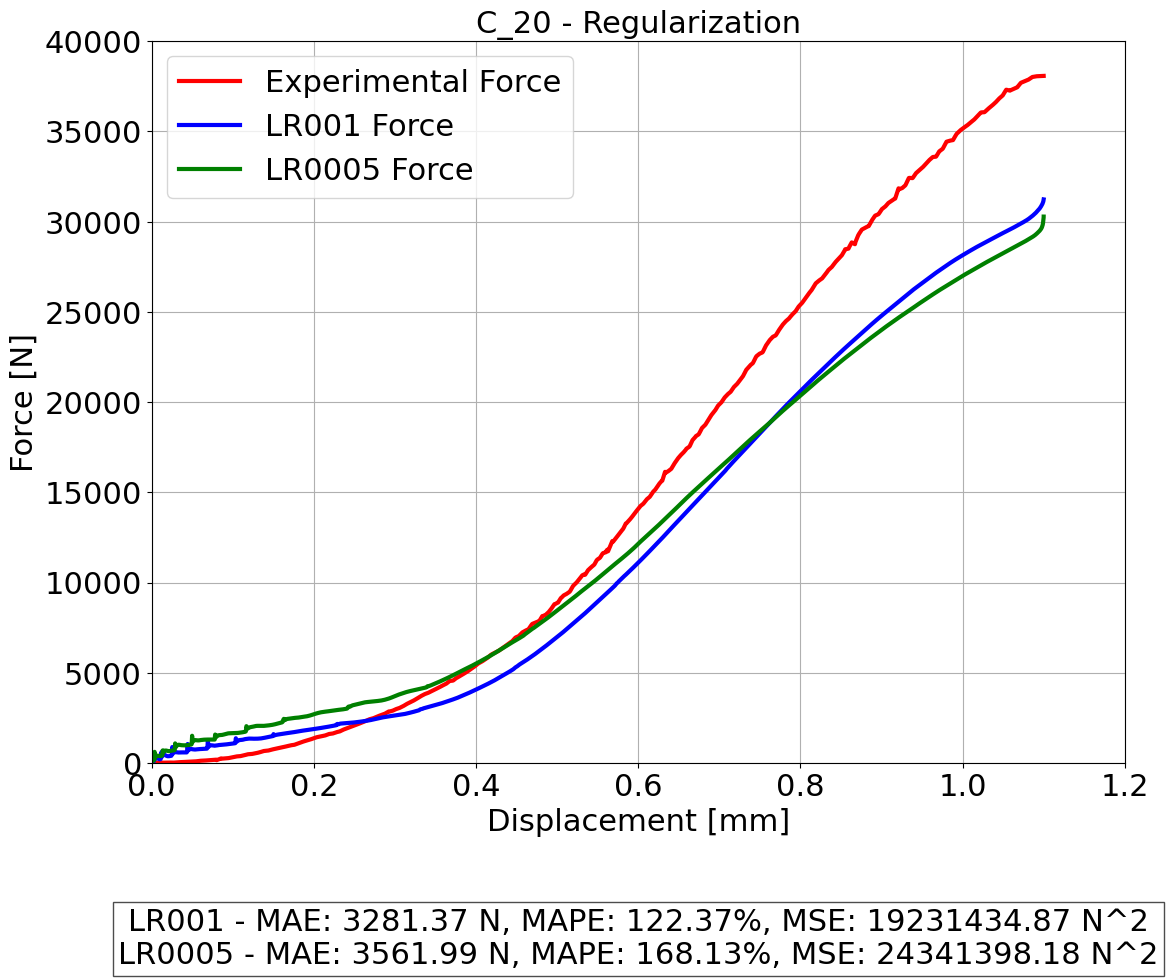
\includegraphics[width=\textwidth]{result_graphics/C_20_RegularizationForce_Comparison.png}
        \end{minipage}
        \hfill
        \begin{minipage}{0.49\textwidth}
            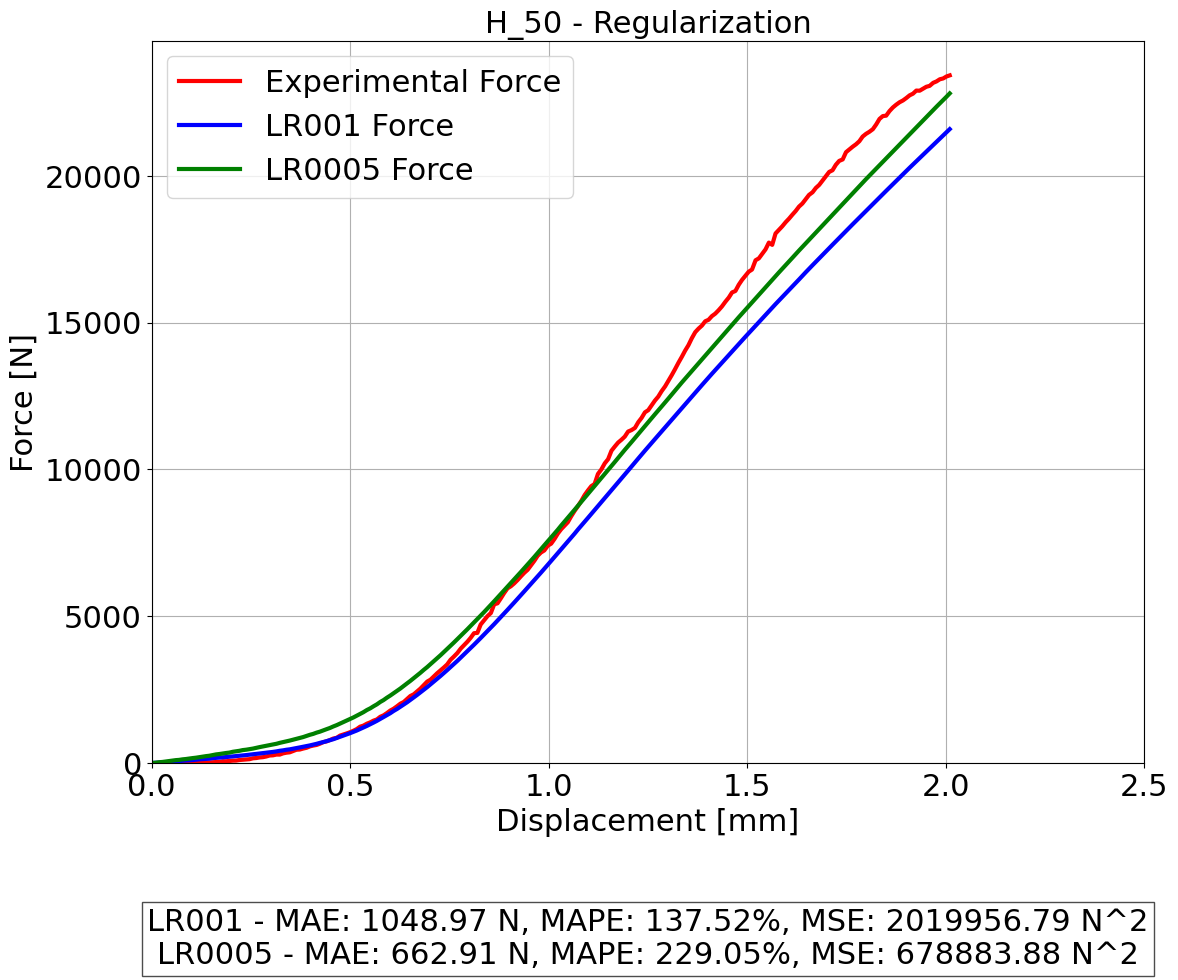
\includegraphics[width=\textwidth]{result_graphics/H_50_RegularizationForce_Comparison.png}
        \end{minipage}
        \caption{Regularization}
        \label{fig:SimpleModel_Training_Regularization_LR0005}
    \end{subfigure}
    
    \vspace{1em} % Adds space between the subfigures
    
    % Second set: Validation Enforce Direction
    \begin{subfigure}[b]{\textwidth}
        \centering
        \begin{minipage}{0.49\textwidth}
            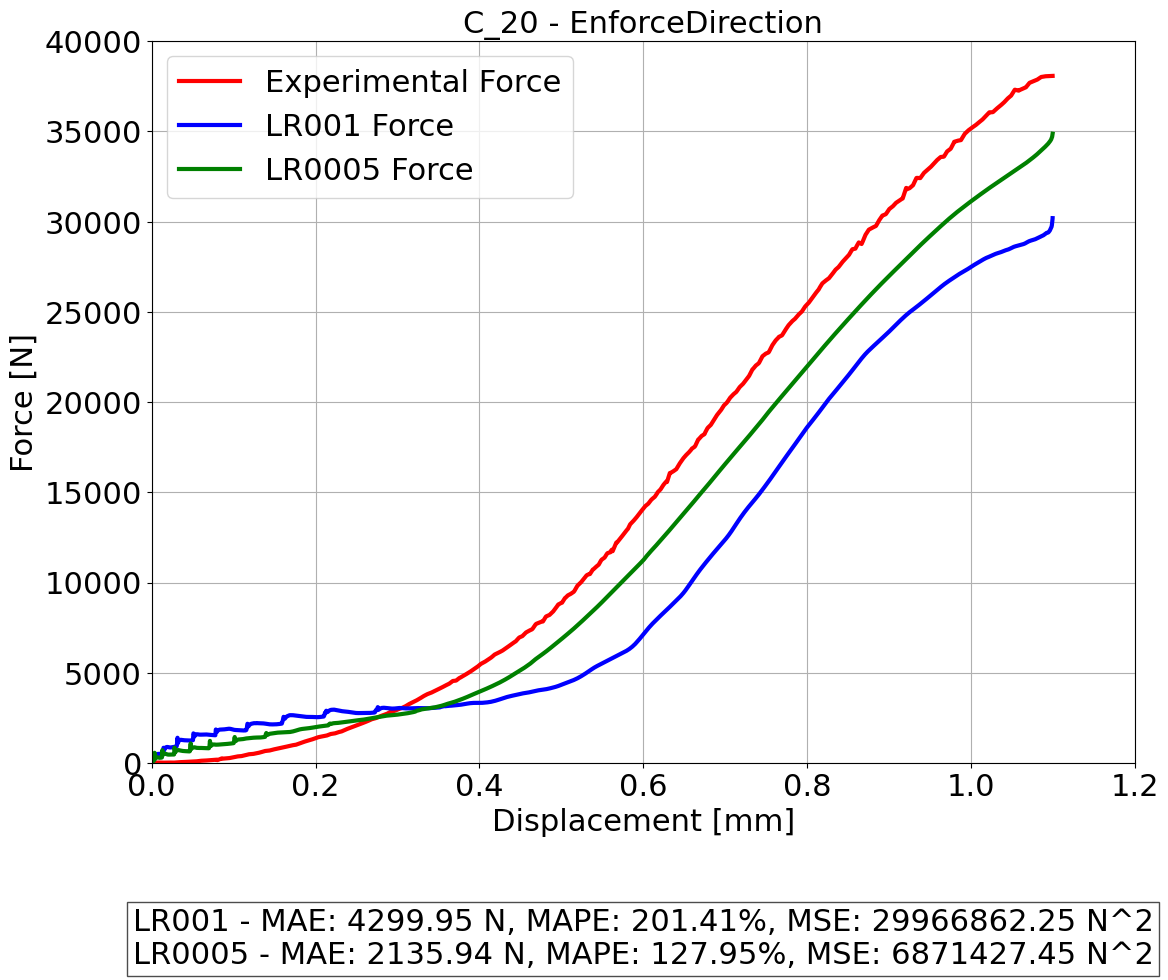
\includegraphics[width=\textwidth]{result_graphics/C_20_EnforceDirectionForce_Comparison.png}
        \end{minipage}
        \hfill
        \begin{minipage}{0.49\textwidth}
            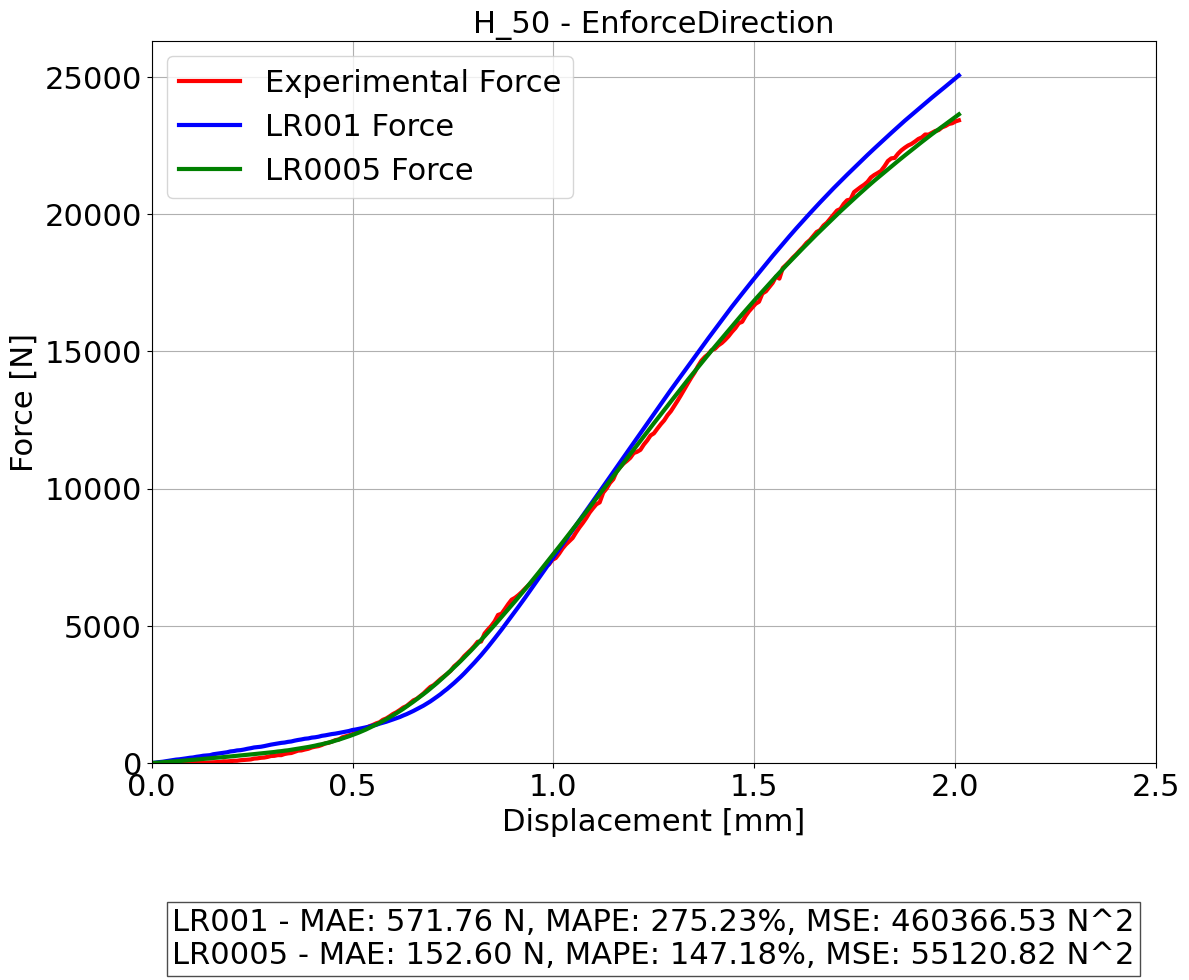
\includegraphics[width=\textwidth]{result_graphics/H_50_EnforceDirectionForce_Comparison.png}
        \end{minipage}
        \caption{Enforce Direction}
        \label{fig:SimpleModel_Training_Regularization_LR001}
    \end{subfigure}
    \caption{Validation results for selected hardening laws}
    \label{fig:Validation_Comparison}
\end{figure}
